% Options for packages loaded elsewhere
\PassOptionsToPackage{unicode}{hyperref}
\PassOptionsToPackage{hyphens}{url}
%
\documentclass[
  ignorenonframetext,
]{beamer}
\usepackage{pgfpages}
\setbeamertemplate{caption}[numbered]
\setbeamertemplate{caption label separator}{: }
\setbeamercolor{caption name}{fg=normal text.fg}
\beamertemplatenavigationsymbolsempty
% Prevent slide breaks in the middle of a paragraph
\widowpenalties 1 10000
\raggedbottom
\setbeamertemplate{part page}{
  \centering
  \begin{beamercolorbox}[sep=16pt,center]{part title}
    \usebeamerfont{part title}\insertpart\par
  \end{beamercolorbox}
}
\setbeamertemplate{section page}{
  \centering
  \begin{beamercolorbox}[sep=12pt,center]{part title}
    \usebeamerfont{section title}\insertsection\par
  \end{beamercolorbox}
}
\setbeamertemplate{subsection page}{
  \centering
  \begin{beamercolorbox}[sep=8pt,center]{part title}
    \usebeamerfont{subsection title}\insertsubsection\par
  \end{beamercolorbox}
}
\AtBeginPart{
  \frame{\partpage}
}
\AtBeginSection{
  \ifbibliography
  \else
    \frame{\sectionpage}
  \fi
}
\AtBeginSubsection{
  \frame{\subsectionpage}
}
\usepackage{amsmath,amssymb}
\usepackage{lmodern}
\usepackage{ifxetex,ifluatex}
\ifnum 0\ifxetex 1\fi\ifluatex 1\fi=0 % if pdftex
  \usepackage[T1]{fontenc}
  \usepackage[utf8]{inputenc}
  \usepackage{textcomp} % provide euro and other symbols
\else % if luatex or xetex
  \usepackage{unicode-math}
  \defaultfontfeatures{Scale=MatchLowercase}
  \defaultfontfeatures[\rmfamily]{Ligatures=TeX,Scale=1}
  \setmainfont[BoldFont = SF Pro Rounded Semibold]{SF Pro Rounded}
  \setmathfont[]{STIX Two Math}
\fi
\usefonttheme{serif} % use mainfont rather than sansfont for slide text
% Use upquote if available, for straight quotes in verbatim environments
\IfFileExists{upquote.sty}{\usepackage{upquote}}{}
\IfFileExists{microtype.sty}{% use microtype if available
  \usepackage[]{microtype}
  \UseMicrotypeSet[protrusion]{basicmath} % disable protrusion for tt fonts
}{}
\makeatletter
\@ifundefined{KOMAClassName}{% if non-KOMA class
  \IfFileExists{parskip.sty}{%
    \usepackage{parskip}
  }{% else
    \setlength{\parindent}{0pt}
    \setlength{\parskip}{6pt plus 2pt minus 1pt}}
}{% if KOMA class
  \KOMAoptions{parskip=half}}
\makeatother
\usepackage{xcolor}
\IfFileExists{xurl.sty}{\usepackage{xurl}}{} % add URL line breaks if available
\IfFileExists{bookmark.sty}{\usepackage{bookmark}}{\usepackage{hyperref}}
\hypersetup{
  pdftitle={444 Lecture 3.6 - The Backward Induction Paradox},
  pdfauthor={Brian Weatherson},
  hidelinks,
  pdfcreator={LaTeX via pandoc}}
\urlstyle{same} % disable monospaced font for URLs
\newif\ifbibliography
\usepackage{graphicx}
\makeatletter
\def\maxwidth{\ifdim\Gin@nat@width>\linewidth\linewidth\else\Gin@nat@width\fi}
\def\maxheight{\ifdim\Gin@nat@height>\textheight\textheight\else\Gin@nat@height\fi}
\makeatother
% Scale images if necessary, so that they will not overflow the page
% margins by default, and it is still possible to overwrite the defaults
% using explicit options in \includegraphics[width, height, ...]{}
\setkeys{Gin}{width=\maxwidth,height=\maxheight,keepaspectratio}
% Set default figure placement to htbp
\makeatletter
\def\fps@figure{htbp}
\makeatother
\setlength{\emergencystretch}{3em} % prevent overfull lines
\providecommand{\tightlist}{%
  \setlength{\itemsep}{0pt}\setlength{\parskip}{0pt}}
\setcounter{secnumdepth}{-\maxdimen} % remove section numbering
\let\Tiny=\tiny

 \setbeamertemplate{navigation symbols}{} 

% \usetheme{Madrid}
 \usetheme[numbering=none, progressbar=foot]{metropolis}
 \usecolortheme{wolverine}
 \usepackage{color}
 \usepackage{MnSymbol}
% \usepackage{movie15}

\usepackage{amssymb}% http://ctan.org/pkg/amssymb
\usepackage{pifont}% http://ctan.org/pkg/pifont
\newcommand{\cmark}{\ding{51}}%
\newcommand{\xmark}{\ding{55}}%

\DeclareSymbolFont{symbolsC}{U}{txsyc}{m}{n}
\DeclareMathSymbol{\boxright}{\mathrel}{symbolsC}{128}
\DeclareMathAlphabet{\mathpzc}{OT1}{pzc}{m}{it}

\setlength{\parskip}{1ex plus 0.5ex minus 0.2ex}

\AtBeginSection[]
{
\begin{frame}
	\Huge{\color{darkblue} \insertsection}
\end{frame}
}

\renewenvironment*{quote}	
	{\list{}{\rightmargin   \leftmargin} \item } 	
	{\endlist }

\definecolor{darkgreen}{rgb}{0,0.7,0}
\definecolor{darkblue}{rgb}{0,0,0.8}

\usepackage[italic]{mathastext}
\usepackage{nicefrac}

\setbeamertemplate{caption}{\raggedright\insertcaption}

%\def\toprule{}
%\def\bottomrule{}
%\def\midrule{}
\usepackage{etoolbox}
\AfterEndEnvironment{description}{\vspace{9pt}}
\AfterEndEnvironment{oltableau}{\vspace{9pt}}
\BeforeBeginEnvironment{oltableau}{\vspace{9pt}}
\AfterEndEnvironment{center}{\vspace{9pt}}
\BeforeBeginEnvironment{tabular}{\vspace{9pt}}
\AfterEndEnvironment{longtable}{\vspace{-6pt}}
\usepackage{booktabs}
\usepackage{longtable}
\usepackage{array}
\usepackage{multirow}
\usepackage{wrapfig}
\usepackage{float}
\usepackage{colortbl}
\usepackage{pdflscape}
\usepackage{tabu}
\usepackage{threeparttable} 
\usepackage{threeparttablex} 
\usepackage[normalem]{ulem} 
\usepackage{makecell}
\usepackage{xcolor}
\usepackage{ulem}

\setlength\heavyrulewidth{0ex}
\setlength\lightrulewidth{0.08ex}

\aboverulesep=0ex
\belowrulesep=0ex
\renewcommand{\arraystretch}{1.2}
\ifluatex
  \usepackage{selnolig}  % disable illegal ligatures
\fi

\title{444 Lecture 3.6 - The Backward Induction Paradox}
\author{Brian Weatherson}
\date{}

\begin{document}
\frame{\titlepage}

\begin{frame}{Plan}
\protect\hypertarget{plan}{}
\begin{itemize}
\tightlist
\item
  To discuss why backward induction isn't quite as popular with
  philosophers as with economists.
\end{itemize}
\end{frame}

\begin{frame}{Reading}
\protect\hypertarget{reading}{}
\begin{itemize}
\tightlist
\item
  No required reading, but if you want to see more, read ``The Backward
  Induction Paradox'' by Philip Pettit and Robert Sugden, \emph{Journal
  of Philosophy} 1989.
\end{itemize}
\end{frame}

\begin{frame}{Backward Induction in Economics}
\protect\hypertarget{backward-induction-in-economics}{}
\begin{itemize}
\tightlist
\item
  I once heard an economist say the biggest controversy about backward
  induction reasoning was whether you say ``backward induction'' or
  ``backwards induction''.
\item
  What he meant, and what's true, is that among mainstream economists,
  this is more controversial than whether the reasoning behind it is
  sound.
\item
  In philosophy there is somewhat more controversy.
\end{itemize}
\end{frame}

\begin{frame}{The Backward Induction Paradox}
\protect\hypertarget{the-backward-induction-paradox}{}
\begin{columns}[c]
\begin{column}{0.48\textwidth}
\begin{figure}
\centering
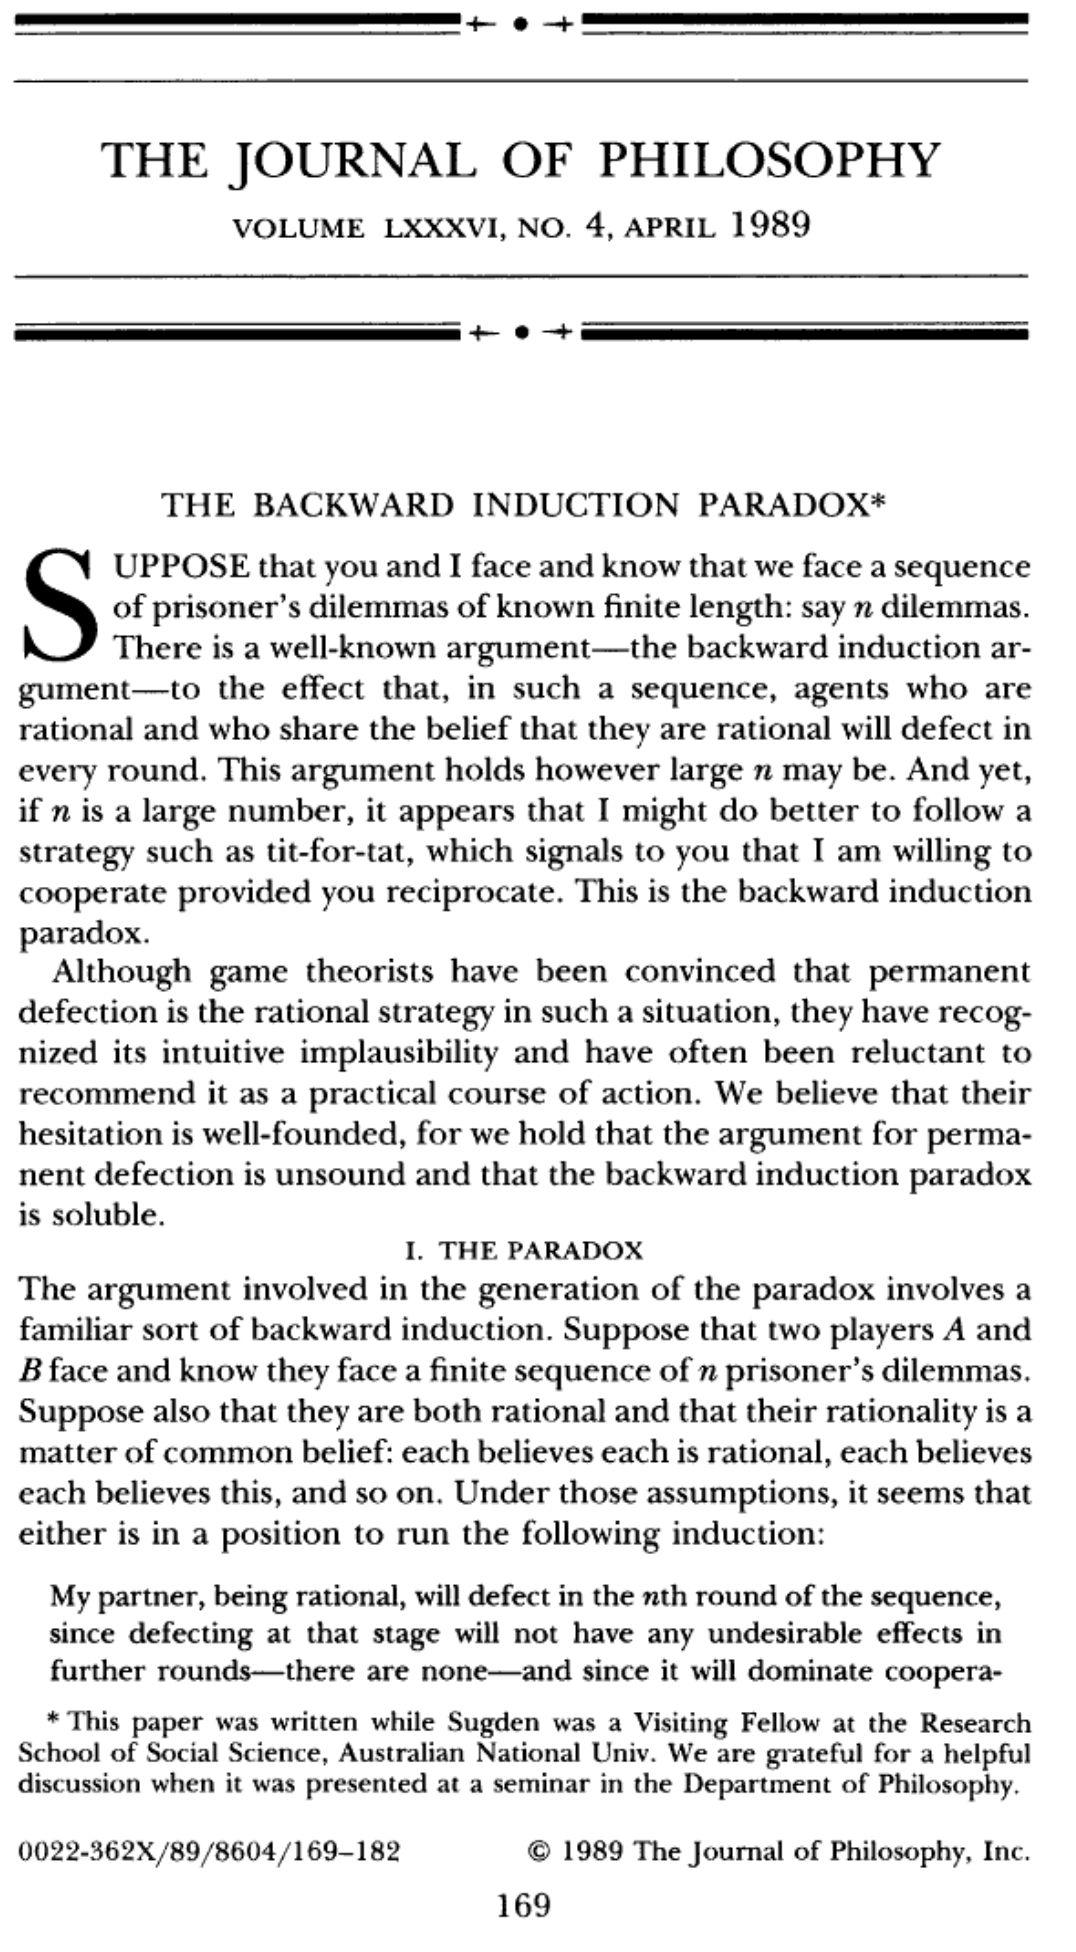
\includegraphics[width=\textwidth,height=0.75\textheight]{images/3_6.png}
\caption{Pettit and Sugden's Paper}
\end{figure}
\end{column}

\begin{column}{0.48\textwidth}
That's in part due to this paper.
\end{column}
\end{columns}
\end{frame}

\begin{frame}{Iterated Prisoners Dilemma}
\protect\hypertarget{iterated-prisoners-dilemma}{}
\begin{itemize}
\tightlist
\item
  It's time to get on the table a game we'll be spending some time on:
  Iterated Prisoners Dilemma.
\item
  It turns out the central event in the history of the study of this
  game happened at the University of Michigan, but that's a story for
  another day.
\item
  A and B will play 100 rounds of the following game.
\end{itemize}

\begin{table}[!h]
\centering
\begin{tabular}[t]{>{}r|cc}
\toprule
 & Coop & Defect\\
\midrule
Coop & 3, 3 & 0, 5\\
Defect & 5, 0 & 1, 1\\
\bottomrule
\end{tabular}
\end{table}
\end{frame}

\begin{frame}{Scoring}
\protect\hypertarget{scoring}{}
\begin{itemize}
\tightlist
\item
  This is still a non-competitive game: they are trying to maximise
  points, not maximise lead over the other.
\item
  But the points add up over all the rounds. (And they don't decay or
  melt.)
\item
  So each party wants to maximise their sum score over 100 plays of the
  game.
\item
  At each play, each party knows what the other did on all the previous
  rounds.
\item
  The strategic form of this is impossibly big; even the two round game
  has 32 strategies per player, so 1024 cells.
\end{itemize}
\end{frame}

\begin{frame}{One Shot Reasoning}
\protect\hypertarget{one-shot-reasoning}{}
At any given round, the following reasoning seems sound.

\begin{enumerate}
\tightlist
\item
  If the other player Cooperates, I'm better off Defecting.
\item
  If the other player Defects, I'm better off Defecting.
\item
  So either way, I'm better off Defecting.
\item
  So, I'm better off Defecting.
\end{enumerate}
\end{frame}

\begin{frame}{Repeated Play}
\protect\hypertarget{repeated-play}{}
But in round one of a repeated game, the following reasoning also looks
sound.

\begin{enumerate}
\tightlist
\item
  The best outcome in the long run is if we both Cooperate as much as
  possible.
\item
  A plausible way to get that would be to signal that I will Cooperate
  if, but only if, the other player does.
\item
  A natural way to implement that is to start Cooperating, then Defect
  when the other player does (this strategy has become known as
  Tit-for-Tat).
\item
  So at round 1 I'll cooperate - if the other player is thinking the
  same way as me, we'll both make a lot of utility, and relative to how
  much there is to gain, it's only a small loss if I'm wrong.
\end{enumerate}
\end{frame}

\begin{frame}{Backward Induction}
\protect\hypertarget{backward-induction}{}
But there is a counter argument.

\begin{enumerate}
\tightlist
\item
  At round 100, there is no signalling value of Cooperating; I just get
  more from Defecting.
\item
  Everyone knows this is true.
\item
  So at round 99, there is no signalling value of Cooperating; the other
  player will Defect at round 100 whatever I do at 99.
\item
  Everyone knows this is true.
\item
  So at round 98, there is no signalling value of Cooperating;\ldots{}
\end{enumerate}
\end{frame}

\begin{frame}{Temporary Conclusion}
\protect\hypertarget{temporary-conclusion}{}
\begin{itemize}
\tightlist
\item
  Backward induction suggests that we should defect every round.
\item
  Eventually there will be no signalling benefit to cooperation, and
  backward induction pushes the moment where that happens back to the
  start of the game.
\end{itemize}
\end{frame}

\begin{frame}{Pettit and Sugden}
\protect\hypertarget{pettit-and-sugden}{}
This reasoning is self-defeating.

\begin{itemize}
\tightlist
\item
  Imagine I'm thinking about cooperating for signalling purposes at
  round one.
\item
  I might worry that the other player will defect come what may at round
  2 because of the backward induction argument.
\item
  But the premises of the backward induction argument imply that I'll
  defect at round 1.
\item
  And at round 2, the other player will know that I did not actually
  defect at round 1.
\item
  So I should only worry if I think the other player will use an
  argument whose premises they know to be false.
\item
  And that's not something to worry about.
\end{itemize}
\end{frame}

\begin{frame}{Short Version}
\protect\hypertarget{short-version}{}
To give up on cooperation requires believing that the other player will
think as follows.

\begin{itemize}
\tightlist
\item
  Game theoretic rationality requires defection at every round, so
  that's what the other player will do from round 3 onwards, so I may as
  well defect.
\item
  And I know that the other player will do what's game theoretically
  rational even though they totally did not do that the very last time I
  interacted with them.
\item
  That's absurd.
\end{itemize}
\end{frame}

\begin{frame}{Game Theorists Respond}
\protect\hypertarget{game-theorists-respond}{}
\begin{itemize}
\tightlist
\item
  You should always think the other player is rational.
\item
  If you observe a departure from rationality, you should assume it is a
  performance error, not a competence error (to use Chomsky's
  terminology).
\item
  Or, to use the terminology of game theorists, you should assume it was
  a ``trembling hand'' error.
\end{itemize}
\end{frame}

\begin{frame}{A Further Puzzle}
\protect\hypertarget{a-further-puzzle}{}
\begin{itemize}[<+->]
\tightlist
\item
  The argument for defecting at round 100 is unaffected by Pettit and
  Sugden's argument, you should totally defect then.
\item
  And I'm not sure that the argument for defecting at round 99 is
  affected either.
\item
  Is round 98 different?
\item
  If you are convinced by their argment that the backward induction
  argument fails in general, when does it start failing?
\end{itemize}
\end{frame}

\begin{frame}{For Next Time}
\protect\hypertarget{for-next-time}{}
We'll end the week looking at a remarkable result involving two player
zero sum games.
\end{frame}

\end{document}
